\documentclass[12pt]{article}
\usepackage{graphicx}
\usepackage[margin=25mm]{geometry}
\usepackage{amsmath}
\usepackage{amssymb}
\usepackage{biblatex}
\usepackage{booktabs}
\usepackage{float}
\usepackage{tabularx}
\renewcommand{\thesubsection}{(\alph{subsection})}
\begin{document}

% Cover Page
\pagebreak
\begin{titlepage}
    \begin{center}
        \vspace*{\fill}
        Lab 7: AC Current and Lighting

        Author: Shaaz Feerasta

        CCID: feerasta

        Student ID: 1704756

        Lab Partner(s): Morgann Reinhart

        PHYS 126, LAB HR81

        TA: Nicolas Concha Marroquin

        Date of Lab: March 13, 2025
        \vspace*{\fill}
    \end{center}
\end{titlepage}

\section{Plots}

\begin{figure}[H]
    \centering
    \begin{minipage}{0.45\textwidth}
        \centering
        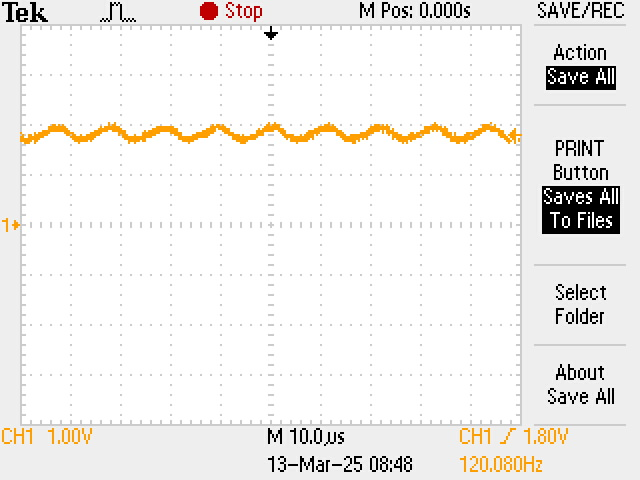
\includegraphics[width=\textwidth]{CFL 1 Graph.jpg}
        \caption{Wavelength of CFL 1 Bulb (X-axis: Time in milliseconds, Y-axis: Voltage in volts)}
        \label{fig:cfl1}
        \end{minipage}
        \hfill
        \begin{minipage}{0.45\textwidth}
        \centering
        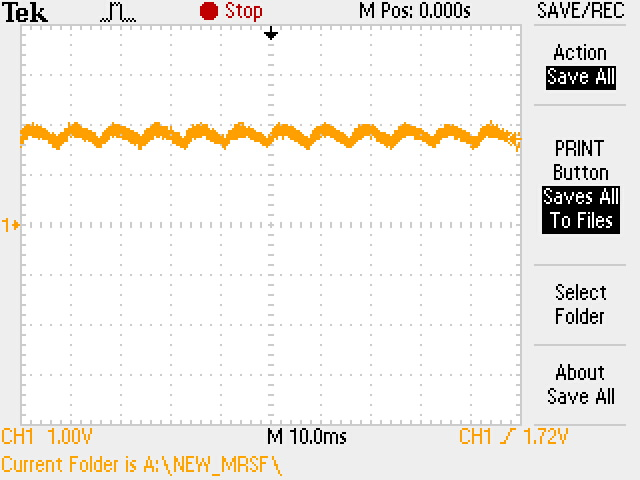
\includegraphics[width=\textwidth]{CFL 2 Graph.jpg}
        \caption{Wavelength of CFL 2 Bulb (X-axis: Time in milliseconds, Y-axis: Voltage in volts)}
        \label{fig:cfl2}
        \end{minipage}
        \vspace{1cm} % Increased vertical space
        \\
        \begin{minipage}{0.45\textwidth}
        \centering
        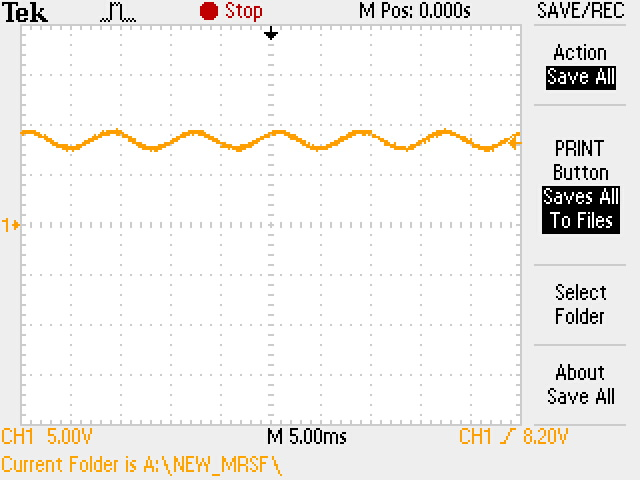
\includegraphics[width=\textwidth]{Incandescent Graph.jpg}
        \caption{Wavelength of Incandescent Bulb (X-axis: Time in milliseconds, Y-axis: Voltage in volts)}
        \label{fig:incandescent}
        \end{minipage}
        \hfill
        \begin{minipage}{0.45\textwidth}
        \centering
        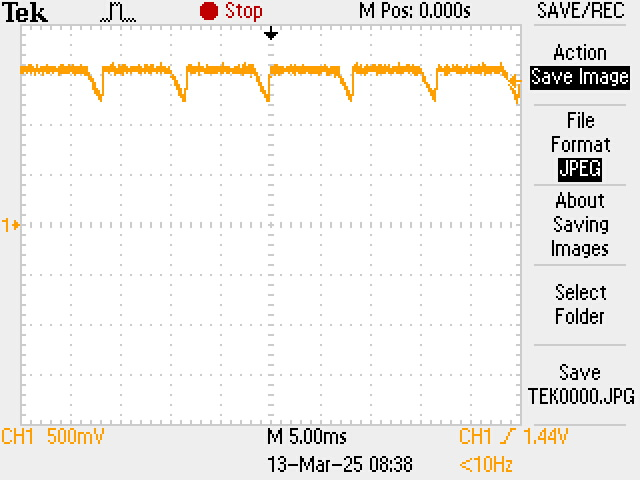
\includegraphics[width=\textwidth]{LED Graph.jpg}
        \caption{Wavelength of LED Bulb (X-axis: Time in milliseconds, Y-axis: Voltage in millivolts and volts)}
        \label{fig:led}
    \end{minipage}
\end{figure}

\section{Incandescent Frequency}

We know that $f = 1/T$, and from our collected data, one wave completes in around $0.008$ seconds.
So, our calculated frequency becomes $\approx 125$ Hz. As for our expected frequency, we know that $V = V_0 \sin (\omega t)$.
So,
\begin{equation*}
    V^2 = V_0^2 \sin^2(\omega t) = V_0^2 \frac{1 - \cos (2 \omega t)}{2} = V_0^2 \frac{1 - \cos (2 (2 \pi f) t)}{2} = V_0^2 \frac{1 - \cos ((2 \pi 2f) t)}{2}
\end{equation*}
We see that our frequency doubles when we square our voltage. Since $P \propto V^2$, for $f = 60$ Hz, our expected
frequency would be $\approx 120$ Hz, which agrees with our experimental frequency.
\section{DC Offset}

There does indeed seem to be a DC offset based on the graph above. We don't really want it to ever reach 0 V, as that means
that there is no voltage going to the bulb, and it would just turn off or dim, and so we need the DC offset.

\section{Tungsten}

Tungsten was chosen due to its high electrical resistivity and high melting point. Meaning, it 
effectively converts the electricity to heat, and doesn't melt either while also resisting high temperatures.

\section{LED Frequency}

Our measured frequency ended up being $\approx 100$ Hz when calculating using the frequency formula. Using the methods above,
we expect our frequency to be around 60 Hz, and so our numbers do not agree. Our voltage does not approach zero here either for the same reasons mentioned previously.
Further, the way LED bulbs work is that it tries to avoid the bottom half of the frequency wave, and if it doesn't go to 0 V,
the technology is doing a good job.

\section{CFL Frequencies}

One of our frequencies for the CFL Bulb was $\approx 91575$ Hz. The other measured frequency was $\approx 113$ Hz. Both frequencies
dip a little towards zero, but none of them actually go to 0 V, based on the graphs.

\section{Steady Output}

Comparing all the graphs, it seems the most steady bulb is the LED bulb. It drops much less often than the other bulbs, but also
shoots back up nearly instantly. It seems to be the most consistent and steady bulb out of all the ones we have experimented with.

\begin{thebibliography}{9}
    \bibitem{labmanual} 
    Department of Physics. \textit{PHYS 126 Lab Manual}. University of Alberta, 2025.

    \bibitem{person}
    TA assisted with the lab, and provided guidance on the data collection and analysis.

    \bibitem{person}
    Lab partner Morgann Reinhart assisted with the data collection and analysis.
    
\end{thebibliography}

\end{document}
